\documentclass[main.tex]{subfiles}
\begin{document}

\section*{Mon Dec 09 2019}

% (BOFGN)

Here is a classification of stars' final fates by initial mass \(M\): 
\begin{enumerate}
    \item \(\num{.8} M_{\odot} < M < \num{2} M_{\odot}\) are low-mass stars: Carbon-Oxygen white dwarves;
    \item \(\num{2} M_{\odot} < M < 6 \divisionsymbol 8 M_{\odot}\) are intermediate-mass stars: Carbon-Oxygen white dwarves;
    \item \(\num{8} M_{\odot} < M < 10 \divisionsymbol 11 M_{\odot}\) are quasi-massive stars: Electron Capture SuperNovae or Oxygen-Neon white dwarves;
    \item \(10 M_{\odot} < M < 30 M_{\odot}\) are massive stars: Core Collapse Supernovae (BH or NS);
    \item \(30 M_{\odot} < M < 100 M_{\odot}\) are massive stars: Black Holes;
    \item \(100 M_{\odot} < M < \num{5e4} M_{\odot}\) are very massive stars: their fate depends on the Helium content in their core: \begin{enumerate}
        \item \(M _{\text{He}} < 65 M_{\odot}\): Pair Instability SuperNovae;
        \item \(65 M_{\odot} < M _{\text{He}} < 133 M_{\odot}\): Pair Creation SuperNovae with no remnant;
        \item \(M _{\text{He}} > 133 M_{\odot}\): Black Holes;
    \end{enumerate}
    \item \(\num{5e4} M_{\odot} < M < \num{e5} M_{\odot}\)  are super massive stars: supernova explosion, with no remnant.
\end{enumerate}

% Massive stars play a key role in several astrophysical and 
% cosmological phaenomena.
% In particular, after their collapse into the supernova, the residual heavy metals and dusts contribute drastically to the formation of new stars.

% Massive stars also are the most important candidate for the explanation of several astrophysical and cosmological issues.

% the existence of black holes, neutron stars, heavy isotopes and gamma ray bursts: that is the reason why we will focus on these stars in our lecture.

Massive stars are pivotal in the description of: 

The \textbf{chemical evolution of galaxies}: they light up (increase the temperature of) the regions of stellar formation, aiding it; they produce most of the heavy elements; they mix up the interstellar medium; they produce neutron stars and black holes.

The \textbf{cosmology} of population III stars: 
reionization of the early (\(z < 5\) ) universe; 
massive remnants such as black holes possibly being the progenitors of Active Galactic Nuclei.

In \textbf{High energy astrophysics}, the production of heavy and long-lived unstable isotopes which can be observed in Gamma Ray Bursts.

% Before doing it for massive stars, we saw a graph picturing the evolution of stars for different mass values: as a rough scheme we have massive stars that become supernovas and then black holes-neutron stars, while low-mass stars slowly turn to red dwarfs.

The most important equations for stellar evolution are the usual ones:
\begin{itemize}
    \item continuity equation 
    %
    \begin{align}
    \dv{r}{m} = \frac{1}{4 \pi r^2 \rho }
    \,,
    \end{align}    
    \item momentum equation 
    %
    \begin{align}
    \dv{P}{m} = - \frac{Gm}{4 \pi r^{4}} - \frac{1}{4 \pi r^2} \dv[2]{r}{t}
    \,,
    \end{align}
    %    
    \item energy transport equation 
    %
    \begin{align}
    \dv{L}{m} = - \frac{Gm}{4 \pi r^4} \frac{T}{P} \nabla
    \,,
    \end{align}
    %
    where \(\nabla\) has contributions from convection, encoded in \(\nabla _{\text{ad}} \), and from radiative transport: 
    %
    \begin{align}
    \nabla _{\text{rad}} = \frac{3 \kappa }{16 \pi acG} \frac{L_r P}{m T^{4}}
    \,,
    \end{align}       
    \item energy conservation equation 
    %
    \begin{align}
    \dv{L}{m} = \epsilon _{\text{nuc}}- \epsilon_{\nu } - T \dv{s}{t}
    \,,
    \end{align}
    %    
    \item chemical species' evolution equation: 
    %
    \begin{align}
    \dv{X_{i}}{t} = A_i \frac{m_u}{\rho } \sum_{j} \qty(r_{ji} - r_{ij})
    \,.
    \end{align}
    %
    
\end{itemize}
%
and we need constitutive relations for the following parameters:
%
\begin{itemize}
    \item pressure $P(\rho,T,X_i)$;
    \item opacity $k(\rho,T,X_i)$;
    \item energy production $\epsilon(\rho,T,X_i)$,
\end{itemize}
%
where \(\rho \) is the density, \(T\) is the temperature and \(X_i\) are the chemical species' mass fractions.

Hereafter we consider very massive stars (\(M > 80 M_{\odot}\)), laying in the main sequence of H-R diagram. In the first time of their life, these stars burn hydrogen in the CNO cycle. When H ends up in the core, it starts the burning of helium in the triple alpha reaction, producing carbon.
Note that in this reaction thermal (i.e. weak-interactions origined) neutrinos are produced.
Then it starts the synthesis of oxygen from carbon, neon from oxygen, magnesium from neon, silicium and iron from magnesium.\footnote{Che al mercato mio padre comprò.}
These elements lay in the star having the heaviest in the core and the others in order of mass. 

\begin{bluebox}
They are elements with mass numbers 1, 4, 12, 16, 20, 24, 28: if helium is present, they are created by adding an \(\alpha \) particle each time. Beryllium (\(A = 8\)) is missing: this is because \ce{^8 Be} is unstable, so the thing which actually happens is that while it is formed an other \(\alpha \) particle comes by and it makes an excited state of \ce{^{12} C} which is close in energy.
\end{bluebox}
    
We said before that pressure is one among the most important variables we shall consider. Its dependence on some other thermodynamical variables is strongly affected by the electron characterization:
%
\begin{subequations}
\begin{align}
P_R &=\frac{aT^4}{3} && \text{in the relativistic case}\\
P_{\text{class}} &=\frac{R\rho T}{\mu} && \text{in the classical perfect-gas case}\\
P_{\text{deg,NR}} &=\rho^{\frac{5}{3}} && \text{for a degenerate gas of non relativistic electrons} \\
P_{\text{deg,R}} &=\rho^{\frac{4}{3}} && \text{for a degenerate gas of relativistic electrons}
\end{align}
\end{subequations}

The main nuclear stages of stellar evolution are 
\begin{enumerate}
    \item core nuclear burning, moving to;
    \item nuclear fuel exhaustion, moving to;
    \item core contraction, moving to;
    \item core heating, back up.
\end{enumerate}

When we get to iron, this process stops.
The contraction raises the temperature: the two are related by a law like \(T _{\text{core}} \propto \rho _{\text{core}}^{1/3}\). 

\subsubsection{Neutrino production}

Now we consider neutrino producion in this phase of the star, since it has been shown that $\epsilon_{\text{nuc}}\approx \epsilon_\nu$, i.e. almost all the power due to nuclear reactions is brought away by neutrinos.
For strong-interaction born neutrinos we have that the free path is
%
\begin{equation}
    l_\nu=\frac{1}{\sigma_\nu n}=\frac{\mu m_u}{\rho\sigma_\nu}\approx 3000 R_{\odot}\,,
\end{equation}
%
since \(\sigma_{\nu } \approx \SI{e-48}{m^{-2}}\).
We are assuming \(\mu \sim 1.3\), and \(\rho \sim \SI{e6}{g/cm^3}\).

This means that neutrinos in average do not interact with the star and can not give back energy to it. This explains the strong neutrinos luminosity (higher than electromagnetic) of almost all the stars, and the consequent mass loss rates.

The main mechanism that can produce weak-interaction or thermal neutrinos are the following:
%
\begin{itemize}
    \item photo-neutrinos production ($\gamma+e^- \to \nu + \bar\nu +e^-$) happens at high temperatures (\(T > \SI{2e8}{K}\)) --- it is basically a Compton process;
    \item pair-neutrinos production ($e^++e^- \to \nu + \bar\nu $) happens at very high temperatures (\(T \gtrsim \SI{e9}{K}\));
    \item plasma-neutrinos production ($\gamma \to \nu + \bar\nu $) happens for degenerate matter with very high density;
    \item bremsstrahlung-neutrinos production (similar, $\gamma \to \nu + \bar\nu $) happens if we have low temperatures but very high density. 
\end{itemize}

In general these processes are very rare in nature, since the probability of emitting a neutrino/antineutrino pair instead of a photon in any process which generally emits a photon is:
%
\begin{equation}
    \frac{\mathbb{P}(\nu\bar\nu)}{\mathbb{P}(\gamma)}=\num{3e-18}\left(\frac{E_\nu}{m_e c^2}\right)^4
\end{equation}
%
but in high-temperature situations (\(E_\nu > \SI{511}{keV}\)) the quantity in parentheses can become larger than 1: the process becomes relevant.
Neutrinos produced anywhere in the core essentially amount to lost energy: if the temperature of the core exceeds \(T_c = \SI{5e8}{K}\), the luminosity of neutrino emission exceeds the electromagnetic one.

For this reason neutrinos are important for the core-cooling process and the speed-up of core reactions.

As we said, during nuclear burning all the (specific) energy produced is brought away by neutrinos, \(\epsilon _{\text{nuc}}\approx \epsilon_{\nu }\): each elements's burning has a characteristic curve \(\epsilon (T)\): these are quite steep, and at a given \(\epsilon \) we need higher and higher temperatures as we reach heavier elements. 
The neutrino curve \(\epsilon_{\nu } (T)\) instead is shallower, and intersects them all: the intersections define the burning temperatures. 

The nuclear timescale is much shorter this way: it is given by 
%
\begin{align}
\tau _{\text{nuc}} = \frac{E _{\text{nuc}}}{\dot{E} _{\text{nuc}}} \approx \frac{E _{\text{nuc}}}{L_{\nu }} \ll \frac{E _{\text{nuc}}}{L}
\,,
\end{align}
%
since \(L_{\nu } \gg L\).
If the cooling happened only electromagnetically the star would need a much longer time to burn.


\begin{figure}[h]
\begin{tabular}{ccccccc}
\Longstack{Burning \\ stage}
& \Longstack{Dominant \\ Process} &
\(T_c\) [\SI{}{keV}] & \(\rho_{c}\) [\SI{}{g/cm^3}] &
\(L_{\gamma }\) [\SI{e4}{} \(L_{\odot}\)] &
\(L_{\nu }/ L_{\gamma }\) & Duration [\SI{}{yr}] \\
\hline
Hydrogen &       H $\rightarrow$ He &   \num{3} & \num{5.9e+00} & \num{2.1} & \num{0.0e+00} & \num{1.2e+07} \\
Helium &    He $\rightarrow$ C, O &  \num{14} & \num{1.3e+03} & \num{6.0} & \num{1.7e-05} & \num{1.3e+06} \\
Carbon &   C $\rightarrow$ Ne, Mg &  \num{53} & \num{1.7e+05} & \num{8.6} & \num{1.0e+00} & \num{6.3e+03} \\
  Neon &   Ne $\rightarrow$ O, Mg & \num{110} & \num{1.6e+07} & \num{9.6} & \num{1.8e+03} & \num{7.0e+00} \\
Oxygen &       O $\rightarrow$ Si & \num{160} & \num{9.7e+07} & \num{9.6} & \num{2.1e+04} & \num{1.7e+00} \\
Silicon &  Si $\rightarrow$ Fe, Ni & \num{270} & \num{2.3e+08} & \num{9.6} & \num{9.2e+05} & \num{1.6e-02} \\
\end{tabular}
\label{tab:massive-star-burning-stages}
\caption{Burning stages of a \(15 M_{\odot}\) star, with neutrino and electromagnetic luminosities.}
\end{figure}

\begin{figure}[H]
\centering
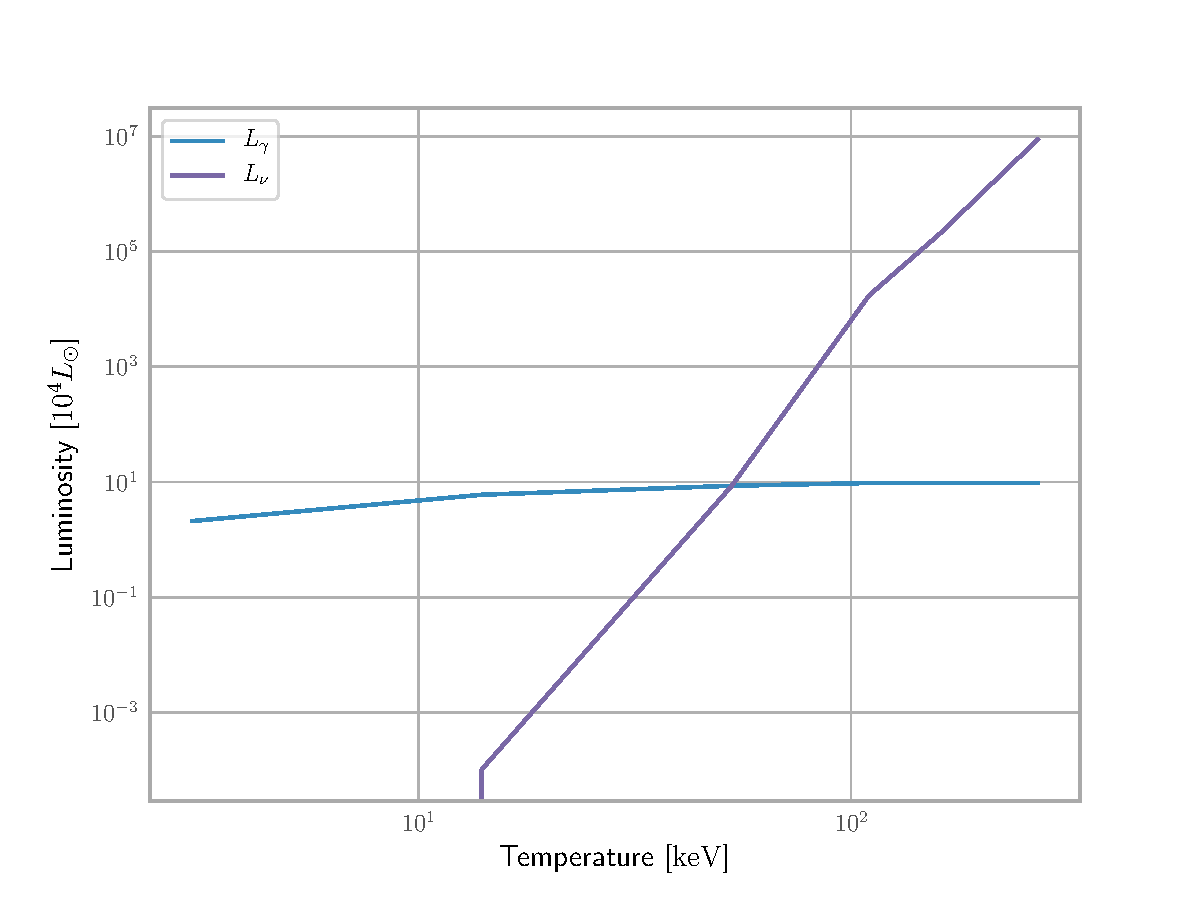
\includegraphics[width=\textwidth]{figures/gamma_nu_luminosities.pdf}
\caption{Electromagnetic and neutrino luminosities as the temperature increases.}
\label{fig:gamma_nu_luminosities}
\end{figure}
    
So, as the later stages of stellar evolution come about, the temperature of the core increases, then neutrino production becomes much more relevant, more energy is lost to it, and therefore the last stages of stellar evolution are much more short-lived than they would be otherwise.

\end{document}
